\pagestyle{fancy}
\fancyhead{}
\fancyhead[L]{Honours DE Workshop 9}
\fancyhead[R]{Winter 2023}

\begin{enumerate}
    \item For part ($a$) consider the following boundary value problem:
    $$y''+\lambda y=0$$
    with:
    $$y(0)-y'(0)=0$$
    $$y(1)+y'(1)=0.$$
    Find the eigenvalues and eigenfunctions to this problem. \\

    Firstly this BVP is in S-L form, and therefore
    $\lambda\in\mathbb{R}$.

    Consider solutions when $\lambda=0$.
    $$\therefore y''=0$$
    Clearly our solutions are linear in this case:
    $$y=a_1 x+a_2.$$
    Now substituting this into our boundary conditions gives:
    $$y(0)-y'(0)=a_2-a_1=0$$
    $$y(1)+y'(1)=a_1+2a_2=0$$
    which implies that $a_1=a_2=0$, so only trivial solutions remain. \\

    So when $\lambda>0$:
    $$y=b_1\sin\lambda^{1/2}x+b_2\cos\lambda^{1/2}x$$
    $$y'=\lambda^{1/2}\bigl(b_1\cos\lambda^{1/2}x-b_2\sin\lambda^{1/2}x\bigl)$$
    and substituting this gives:
    $$y(0)-y'(0)=b_2-\lambda^{1/2}b_1=0.$$
    $$\therefore b_2=\lambda^{1/2}b_1$$
    Our solution can then be written as:
    $$y=b_1\bigl(\sin\lambda^{1/2}x+\lambda^{1/2}\cos\lambda^{1/2}x\bigl)$$
    and its derivative:
    $$y'=b_1\bigl(\lambda^{1/2}\cos\lambda^{1/2}x-\lambda\sin\lambda^{1/2}x\bigl).$$

    \newpage

    The other boundary condition gives:
    \begin{align*}
        y(1)+y'(1)
        &=b_1\bigl(\sin\lambda^{1/2}+\lambda^{1/2}\cos\lambda^{1/2}\bigl)
        +b_1\bigl(\lambda^{1/2}\cos\lambda^{1/2}-\lambda\sin\lambda^{1/2}\bigr) \\
        &=b_1\Bigl((1-\lambda)\sin\lambda^{1/2}+2\lambda^{1/2}\cos\lambda^{1/2}\Bigr) \\
        &=0
    \end{align*}
    which implies the following relation:
    $$\tan\lambda_n^{1/2}=\frac{2\lambda_n^{1/2}}{\lambda_n-1}$$
    with its corresponding eigenfunction:
    $$\phi_n(x)=k_n\bigl(\sin\lambda_n^{1/2}x+\lambda_n^{1/2}\cos\lambda_n^{1/2}x\bigr).$$ \\

    Now consider solutions when $\lambda<0$:
    $$y=c_1\cosh\lambda^{1/2}x+c_2\sinh\lambda^{1/2}x.$$
    Taking derivatives gives the following:
    $$y'=\lambda^{1/2}\bigl(c_1\sinh\lambda^{1/2}x+c_2\cosh\lambda^{1/2}x\bigr).$$
    Now the first boundary condition gives:
    $$y(0)-y'(0)=c_1-\lambda^{1/2}c_2=0$$
    or that
    $$c_1=\lambda^{1/2}c_2.$$
    Rewriting our solutions:
    $$y=c_2\bigl(\lambda^{1/2}\cosh\lambda^{1/2}x+\sinh\lambda^{1/2}x\bigr)$$
    $$y'=c_2\bigl(\lambda\sinh\lambda^{1/2}x+\lambda^{1/2}\cosh\lambda^{1/2}x\bigr).$$
    Using the second boundary condition:
    \begin{align*}
        y(1)+y'(1)
        &=c_2\bigl(\lambda^{1/2}\cosh\lambda^{1/2}+\sinh\lambda^{1/2}\bigr)
        +c_2\bigl(\lambda\sinh\lambda^{1/2}+\lambda^{1/2}\cosh\lambda^{1/2}\bigr) \\
        &=c_2\bigl(2\lambda^{1/2}\cosh\lambda^{1/2}
        +(\lambda+1)\sinh\lambda^{1/2}\bigr) \\
        &=0
    \end{align*}
    and so we end up with the following relation:
    $$\tanh\lambda_n^{1/2}=-\frac{2\lambda_n^{1/2}}{\lambda_n+1}$$
    with eigenfunction:
    $$y=c_2\bigl(\lambda_n^{1/2}\cosh\lambda_n^{1/2}x+\sinh\lambda_n^{1/2}x\bigr).$$

    \newpage

    For part ($b$)($i$) we examine integrating factors. Define:
    $$\mu(x)=\frac{1}{P(x)}\exp\left[\int_{x_0}^{x}\frac{Q(s)}{P(s)}\dd s\right]$$
    to be the integrating factor to the following ODE:
    $$P(x)y''+Q(x)y'+R(x)y=0.$$
    Because by construction we have that:
    $$\bigl[\mu Py'\bigr]'=\mu Py''+\mu Qy'$$
    therefore multiplying our original ODE yields the following:
    $$\bigl[\mu Py'\bigr]'+\mu Ry=0.$$
    We now consider some examples of this method. For part ($b$)($ii$)(1):
    $$y''-2xy'+\lambda y=0$$
    may be converted into the following form:
    $$\bigl[\exp(-x^2)y'\bigr]'+\lambda\exp(-x^2)y=0.$$
    For part ($b$)($ii$)(2):
    $$x^2 y''+xy'+(x^2-v^2)y=0$$
    gives:
    $$\bigl[(x^2-v^2)^{1/2}y'\bigr]'+\frac{(x^2-v^2)^{3/2}}{x^2}y=0.$$
    Finally for part ($b$)($ii$)(3):
    $$(1-x^2)y''-xy'+\alpha^2 y=0$$
    we have that
    $$\bigl[(1-x^2)^{1/2}y'\bigr]'+\alpha^2(1-x^2)^{-1/2}y=0.$$

    \newpage

    For part ($c$) firstly find the \underline{normalised}
    eigenfunctions to:
    $$y''+\lambda y=0$$
    with boundary conditions $y'(0)=0$ and
    $$y(1)+y'(1)=0.$$ \\

    This is of S-L form:
    $$-y''=\lambda y$$
    with $r(x)=1$. (This will be important for inner products.)

    Now the eigenvalues with be real and we consider three cases. \\

    If $\lambda=0$:
    $$y'=a_1x+a_2$$
    and using our boundary conditions only trival solutions remain. \\

    If $\lambda>0$:
    $$y=b_1\sin\lambda^{1/2}x+b_2\cos\lambda^{1/2}x$$
    $$y'=\lambda^{1/2}\bigl(b_1\cos\lambda^{1/2}x-b_2\sin\lambda^{1/2}x\bigl)$$
    which after solving for boundary conditions gives:
    $$\lambda_n^{-1/2}=\tan\lambda^{1/2}$$
    $$\phi_n(x)=k_n\cos\lambda^{1/2}x$$
    which we can see have nontrivial eigenvalues. \\\\
    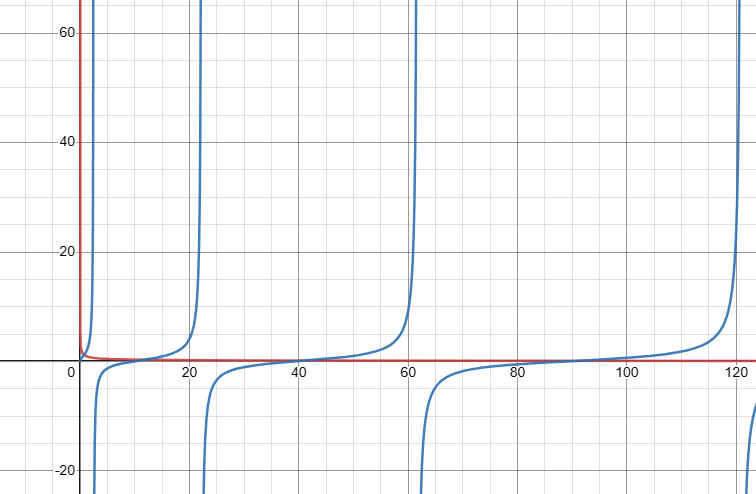
\includegraphics[scale=0.4]{w09_1c.png}

    \newpage
    Now if $\lambda<0$ we have:
    $$y=c_1\cosh\lambda^{1/2}x+c_2\sinh\lambda^{1/2}x.$$
    $$y'=\lambda^{1/2}\bigl(c_1\sinh\lambda^{1/2}x+c_2\cosh\lambda^{1/2}x\bigr).$$
    and substituting for boundary conditions gives:
    $$\tanh\lambda^{1/2}=-\lambda^{1/2}$$
    $$\phi_n(x)=m_n\sinh\lambda^{1/2}x.$$
    But a plot shows that only trivial eigenvalues exists for this case. \\\\
    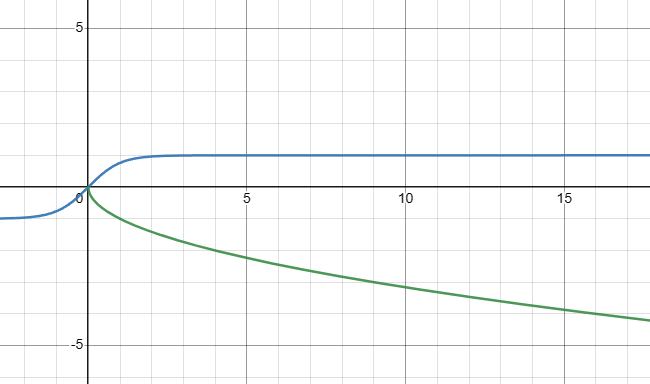
\includegraphics[scale=0.4]{w09_1c_1.png}

    And therefore we conclude that the only nontrivial solutions to our S-L problem is:
    $$\lambda_n^{-1/2}=\tan\lambda^{1/2}$$
    $$\phi_n(x)=k_n\cos\lambda^{1/2}x.$$
    We now need to find the normalisation constant $k_n$:
    \begin{align*}
        \langle\phi_n, \phi_n \rangle
        &=\int_{0}^{1}k_n^2\cos^2\lambda_n^{1/2}x\dd x \\
        &=\frac{1}{2}k_n^2
        \left[1+\frac{1}{2\lambda_n^{1/2}}\sin2\lambda_n^{1/2}\right] \\
        &=1
    \end{align*}
    in Hilbert space $L^2([0,1],1)$. Therefore we have that:
    $$k_n=\left(\frac{4\lambda_n^{1/2}}{2\lambda_n^{1/2}+\sin2\lambda_n^{1/2}}\right)^{1/2}.$$

    \newpage

    The question now asks us to find a series expansion for $f(x)=x$ in terms
    of our orthonormal eigenfunction basis. So we have that:
    $$f_\phi(x)=\sum_{n=1}^{\infty}c_n\phi_n(x)$$
    where $f_\phi=x$ and it remains to compute the coefficients.

    So integrating on both sides gives:
    \begin{align*}
        \int_{0}^{1}r(x)\phi_m(x)f(x)\dd x
        &=\int_{0}^{1}r(x)\phi_m(x)
        \sum_{n=1}^{\infty} c_n\phi_n(x)\dd x \\
        &=\sum_{n=1}^{\infty} c_n
        \int_{0}^{1}r(x)\phi_m(x)\phi_n(x)\dd x \\
        &=\sum_{n=1}^{\infty} c_n\delta_{mn} \\
        &=c_m
    \end{align*}
    and since $r(x)=1$ we obtain the following:
    \begin{align*}
        c_n
        &=\int_{0}^{1}\phi_n(x)f(x)\dd x \\
        &=\int_{0}^{1}k_n y_n(x)f(x)\dd x \\
        &=k_n\int_{0}^{1}y_n(x)f(x)\dd x.
    \end{align*}
    From the previous page we have:
    $$\phi_n(x)=k_n\cos\lambda^{1/2}x$$
    and so substituting everything in:
    \begin{align*}
        c_n
        &=k_n\int_{0}^{1}x\cos\lambda^{1/2}x\dd x \\
        &=k_n\left(\frac{1}{\lambda_n^{1/2}}\sin\lambda_n^{1/2}
        +\frac{1}{\lambda_n}\cos\lambda_n^{1/2}-\frac{1}{\lambda_n}\right)
    \end{align*}
    where we have:
    $$k_n=\left(\frac{4\lambda_n^{1/2}}{2\lambda_n^{1/2}+\sin2\lambda_n^{1/2}}\right)^{1/2}.$$

    \newpage

    \item Solve the following:
    $$y''+2y=-x$$
    with boundary conditions:
    $y(0)=0$ and $y'(1)=0$. \\

    First consider the corresponding homogeneous S-L problem:
    $$-y''=\lambda y$$
    with the same boundary conditions. If $\lambda\leq0$ we only have trivial solutions.
    Hence assume $\lambda>0$. After solving and substituting boundary conditions we get:
    $$\phi_n(x)=k_n\sin\lambda_n^{1/2}$$
    $$\lambda_n^{1/2}=(2n+1)\frac{\pi}{2}$$
    with normalisation constant:
    $$k_n=\sqrt{2}\left(1-\frac{1}{2\lambda^{1/2}}\sin2\lambda^{1/2}\right)^{-1/2}.$$ \\

    Rewriting our original ODE in S-L form:
    $$-y''=\mu r(x) y+f(x)$$
    and hence this ODE has $\mu=2$, $r(x)=1$ and $f(x)=x$. So using our homogeneous eigenfunctions
    we can write the solution as a sum of our eigenfunctions:
    $$y(x)=\sum_{n=1}^{\infty}b_n\phi_n(x)$$
    which after substituting into our ODE we get:
    $$\sum_{n=1}^{\infty}\lambda_n \phi_n(x)
    =\sum_{n=1}^{\infty}\mu\phi_n(x)+x.$$
    $$\therefore\sum_{n=1}^{\infty}b_n(\lambda_n-\mu)\phi_n(x)=x.$$
    But we can also expand $f(x)=x$ in terms of our eigenfunctions:
    $$f(x)=\sum_{n=1}^{\infty}c_n\phi_n(x)$$
    and so
    $$c_n=\int_{0}^{1}\phi_n(x)f(x)\dd x$$
    with the equality:
    $$b_n=\frac{c_n}{\lambda_n-\mu}.$$
    
    \newpage

    The only thing let is to compute $c_n$:
    \begin{align*}
        c_n
        &=\int_{0}^{1}k_n y_n(x)f(x)\dd x \\
        &=k_n\int_{0}^{1}x\sin\lambda_n^{1/2}x\dd x \\
        &=k_n\left(-\frac{1}{\lambda_n^{1/2}}\cos\lambda_n^{1/2}
        +\frac{1}{\lambda_n}\sin\lambda_n^{1/2}\right)
    \end{align*}
    with
    $$k_n=\sqrt{2}\left(1-\frac{1}{2\lambda_n^{1/2}}\sin2\lambda_n^{1/2}\right)^{-1/2}.$$
    Then the solution to our ODE is
    $$y(x)=\sum_{n=1}^{\infty}b_n\phi_n(x)$$
    where
    $$b_n=\frac{k_n}{\lambda_n-2}\left(-\frac{1}{\lambda_n^{1/2}}\cos\lambda_n^{1/2}
    +\frac{1}{\lambda_n}\sin\lambda_n^{1/2}\right)$$
    $$k_n=\sqrt{2}\left(1-\frac{1}{2\lambda_n^{1/2}}\sin2\lambda_n^{1/2}\right)^{-1/2}$$
    and
    $$\phi_n(x)=k_n\sin\lambda_n^{1/2}$$
    $$\lambda_n^{1/2}=(2n+1)\frac{\pi}{2}.$$
\end{enumerate}